The figure \ref{fig:component_diagram} represents the Safestreets component diagram. Each of the components are wrapped inside a specific box that indicates the subsystem in which they belong to.
\newline Subsystems are groups of components which perform similar operations: this boxing technique is a multilayer logical division that can be useful in order to categorize the components and the whole system at different layers of abstraction.
\newline For the sake of simplicity, the component diagram pictures the application layer (backend) of the system and not the mobile and web app structures. The business logic and core functions are fully contained in the application layer and therefore only that relevant part of the Safestreets system has been characterized.
\begin{figure}[H]
    \centering
    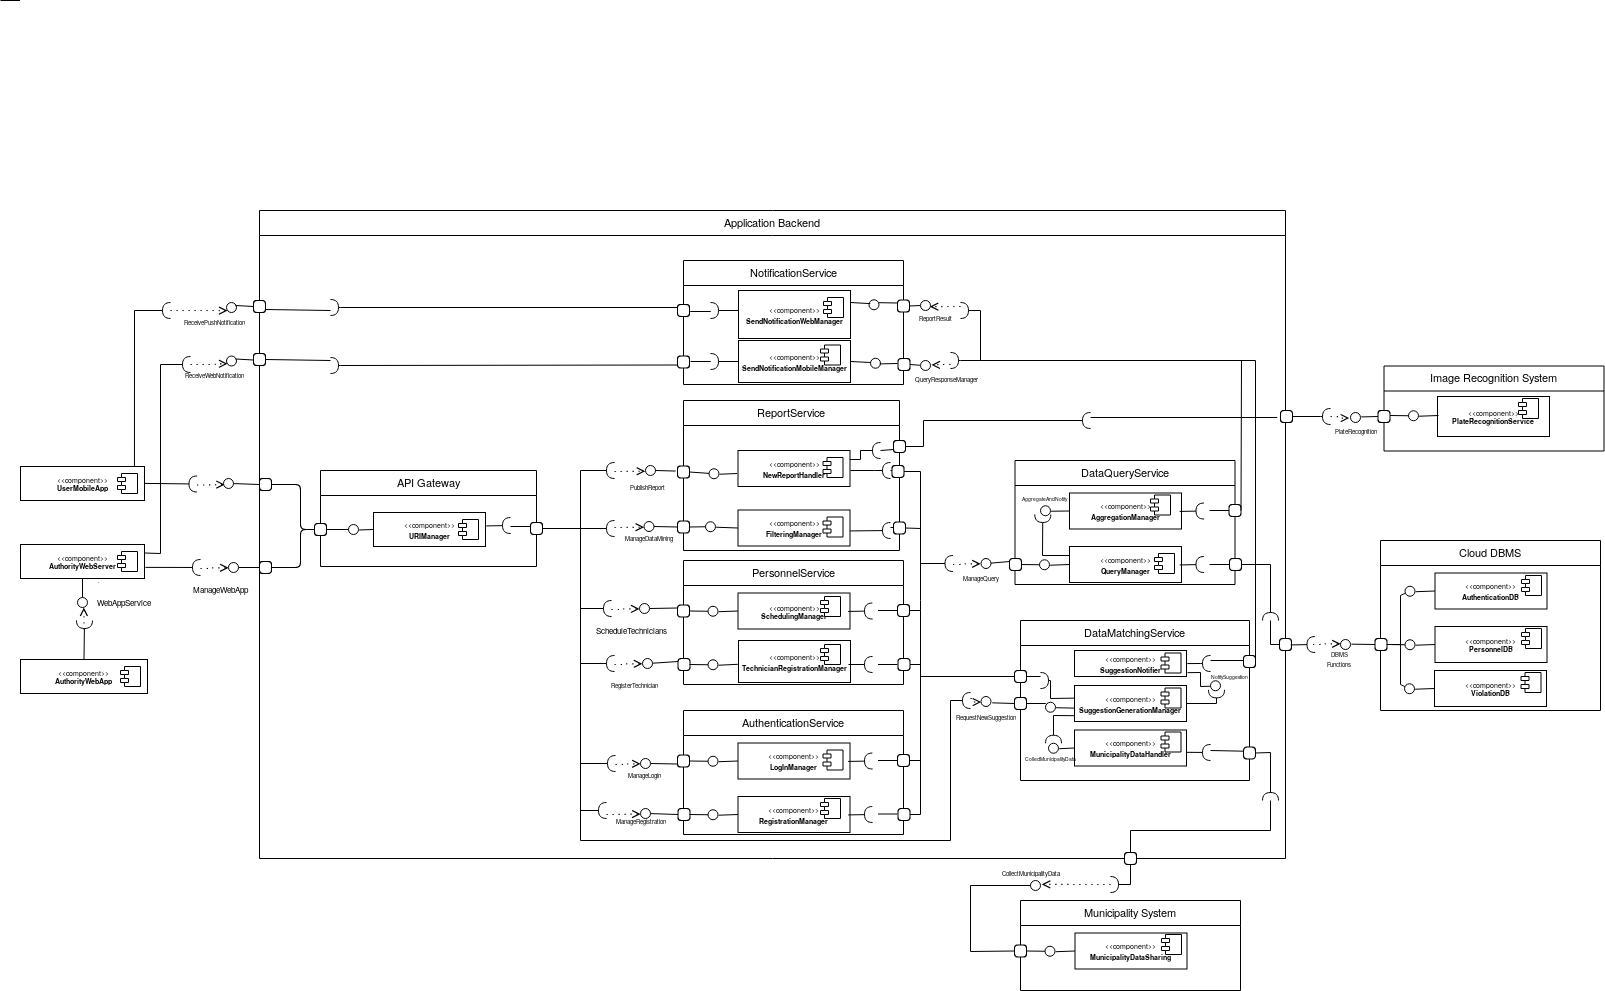
\includegraphics[width=1.1\textwidth]{UML_diagrams/component_uml_safestreets}
    \caption{Component UML diagram}
    \label{fig:component_diagram}
\end{figure}
From the figure \ref{fig:component_diagram} it is possible to identify several subsystem of the application backend system. Here it is a detailed list of the subsystems:
\begin{itemize}
    \item \textbf{API Gateway}: this subsystem is responsible for handling all the request coming from the frontend applications (web and mobile) and routing them into the appropriate components;
    \item \textbf{ReportService}: this subsystem is responsible for handling all the operations related to the violation reports. It interacts directly with the image recognition service in order to retrieve the license plate transctiptions;
    \item \textbf{PersonnelService}: this subsystem is responsible for handling all the operations related to the personnel management, such as registering new technicians and scheduling them to reports. This subsystem is accessible only by LSA accounts;
    \item \textbf{AuthenticationService}: this subsystem is responsible for handling the login and registration operations;
    \item \textbf{SuggestedInterventionServie}: this subsystem is responsible for handling the operation related to the request of suggested interventions. It interacts directly with the municipality system in order to retrieve car accident information;
    \item \textbf{DataQueryService}: this subsystem is responsible for handling all the operations that requires a database interaction. It is responsible for interacting with the Cloud DBMS in order to retrieve all the information required by the application backend;
    \item \textbf{NotificationService}: this subsystem is responsible for forwarding results of the computation to the frontend applications (web and mobile).
\end{itemize} 
Here it is a detailed explanation for each of the components shown in the component diagram:
\begin{itemize}
    \item \textbf{AuthorityWebApp}: this component represents the web application that LSAs and technicians are supposed to use in order to perform any operation with the Safestreets system. In particular, the web app is the end-user application, therefore it is only a frontend interface;
    \item \textbf{AuthorityWebServer}: this component represents the web server that hosts the web application used by LSAs and technicians. The web server receives all the HTTP requests from the AuthorityWebApp and forwards them to the application backend system. Moreover, the web server notifies the web application when the responses of the previous requests are forwarded from the Notification Service;
    \item \textbf{UserMobileApp}: this component represents the mobile application which users interacts with. When users need to perform a specific function offered by the system, the mobile application automatically forwards it to the application backend system. Moreover, the application is always listening for push notifications coming from the Notification service in case one of the previously reported violation is updated by the technicians;
    \item \textbf{URIManager}: this component is responsible for forwarding the requests coming from the frontend system to the backend subsystem which is able to handle the specific request. This routing is possible thanks to the target URI of the frontend request, that uniquely identify the associated component of the application backend system;
    \item \textbf{NewReportHandler}:this component handles the newly reported violation that are forwarded from the URIManager. The NewReportHandler is responsible for checking the correctness of the new reported data and to delegate the plate recognition to the PlateRecognitionService which is external with respect to the Safestreets system. Once the report has been verified and the plate transctiption has been gathered, the report is forwarded to the QueryManager, specifying an insertion request;
    \item \textbf{PlateRecognitionService}: this component is external from the Safestreets system. It has been created for graphical purposes and it is treated as a black box: given a plate image, it is able to transcribe the license plate and give it back to the NewReportHandler;
    \item \textbf{FilteringManager}: this component is responsible for formulating mining operations. The URIManager forwards the mining information to the FilteringManager, which gathers and aggregate all the query parameter and forwards the formally complete query to the QueryManager specifying a select request;
    \item \textbf{SchedulingManager}: this component is responsible for performing the association between technicians and reports. This component can be invoked only if the requesting account is a LSA. After a series of checks, the verified requests is wired into a query and it is forwarded to the QueryManager specifying an insert request;
    \item \textbf{TechnicianRegistrationManager}: this component is responsible for the registration of new technicians into the system. This component can be invoked only if the requesting account is a LSA. The new technicians are directly associated to the requesting LSA. All the needed queries are formulated and forwarded to the QueryManager specifying for each query an insert request;
    \item \textbf{LoginManager}: this component is responsible for logging into the system both users and authorities. The request forwarded from the URIManager contains a username and a password: an hash is calculated from the password and the (username, hash) tuple is wired into a select query which will be forwarded to the QueryManager, specifying a login request;
    \item \textbf{RegistrationManager}: this component is responsible for registering new users to the system. After a series of checks, the registration request is wired into a query and forwarded to the QueryManager specifying an insert request;
    \item \textbf{SuggestionGenerationManager}: this component is responsible for generating suggested interventions when an LSA requests it. The URIManager forwards the generic request of suggestion generation and the system automatically performs the following sequence of actions: 
    \begin{itemize}
        \item If not cached, formulate a query on the LSA competence area, asking for the most frequent categories of violations occured in that set of streets;
        \item Save on a local cache the information;
        \item Formulate a data request of car accident to the MunicipalityDataHandler and retrieve the response;
        \item Aggregate the two kind of data and compute suggested interventions;
        \item Forward the suggested interventions to the SuggestionNotifier.
    \end{itemize}
    \item \textbf{MunicipalityDataHandler}: this component is responsible for taking the data requests coming from the SuggestionGenerationManager and formulate them into the municipality standard. Once this operation is performed, the request is forwarded to the MunicipalityDataSharing interface together with an authentication token provided by the municipality. If the token has expired, a new one is requested and the operation is repeated. When data is provided, it is backpropagated to the SuggestionGenerationManager;
    \item \textbf{MunicipalityDataSharing}: this component is external from the Safestreets system. It has been created for graphical purposes and it is treated as a black box: when a formally correct request is received together with an authentication token, the MunicipalityDataSharing system forwards the requested information to the MunicipalityDataHandler;
    \item \textbf{SuggestionNotifier}: this component is responsible for forwarding the suggested interventions set to the LSA account web app through the SendNotificationWebManager;
    \item \textbf{QueryManager}: this component is responsible for interacting with the data layer of the Safestreets system. The QueryManager is able to connect directly with the Cloud DBMS and perform queries on the several databases of the Safestreets system. When this component receives query information, it acts as following: 
    \begin{itemize}
        \item Perform queries depending on their kinds: 
        \begin{itemize}
            \item Insert: tries to insert the specified data into the database;
            \item Select: retrieve the filtered data;
            \item Login: retrieve the specified data and checks wether the result contains at least one correspondency;
        \end{itemize}
        \item Forwards the result to the AggregationManager.
    \end{itemize}
    \item \textbf{AuthenticationDB}: this component is external from the Safestreets system. It has been created for graphical purposes and it is treated as a black box: it contains all the information associated to the Safestreets accounts;
    \item \textbf{PersonnelDB}: this component is external from the Safestreets system. It has been created for graphical purposes and it is treated as a black box: it contains all the information associated to personnel of the authorities: any kind of association between LSAs and technicians relation and the technicians schedules;
    \item \textbf{ViolationDB}: this component is external from the Safestreets system. It has been created for graphical purposes and it is treated as a black box: it contains all the information associated to the violation reports;
    \item \textbf{AggregationManager}: this component is responsible for packing the retrieved data from the QueryManager into a standard format and forward it to the SendNotificationWebManager or SendNotificationMobileManager depending on the kind of account that performed that specific operation;
    \item \textbf{SendNotificationWebManager}: this component is responsible for forwarding the result of the requested operation to the web application of the account whom requested such operations;
    \item \textbf{SendNotificationMobileManager}: this component is responsible for forwarding the result of the requested operation to the mobile application of the account whom requested such operations;
\end{itemize}